\documentclass{article}

\usepackage{graphicx}
\usepackage{float}
\usepackage{booktabs}
\usepackage{microtype}
\usepackage[ngerman]{babel}
\usepackage[utf8]{inputenc}
\usepackage{csquotes}
\usepackage{seqsplit}
\usepackage[hidelinks]{hyperref}

\emergencystretch=2em

\usepackage[
    backend=biber,
    style=apa
]{biblatex}

\addbibresource{./extra/literatur.bib}

\setcounter{secnumdepth}{3}
\setcounter{tocdepth}{3}

\begin{document}

% Titelseite

% ======================
% Deckblatt
% ======================

\begin{titlepage}
  \centering
  \begin{flushleft}
  
\includegraphics[width=3.5cm]{./bilder/uni_logo.png}
  \end{flushleft}
\vspace{0.5cm}

  {\Large \textbf{Universität Bremen} \par}
  \vspace{0.3cm}
  {\large Fachbereich 3 - Mathematik und Informatik \par}

  \vspace{1.2cm}

  {\large Semester: Sommersemester 2026 \par}
  \vspace{0.2cm}
  {\large Dozentin: Michaela Kümpel \par}
  \vspace{0.2cm}

  \vfill

  {\LARGE \textbf{Bachelorprojekt Rehab} \par}
  \vspace{0.3cm}
  {\Large \textbf{Abschlussbericht} \par}

  \vfill

  \begin{tabular}{@{}l@{\hspace{1em}}l@{}}
    \multicolumn{2}{@{}l}{\textbf{Gruppenmitglieder:}} \\
    Nadine Albers           & \texttt{albersn@uni-bremen.de} \\
    Mika Schneider          & \texttt{mikaales@uni-bremen.de} \\
    Louis Unruh             & \texttt{lunruh@uni-bremen.de} \\
    Parizoda Alimukhamedova & \texttt{pa\textunderscore al@uni-bremen.de} \\
    Khaled Almasri          & \texttt{almasri@uni-bremen.de} \\
    Amjad Faham             & \texttt{amjfah@uni-bremen.de} \\
    Daniel Fetzer           & \texttt{fetzerd@uni-bremen.de} \\
    Bjarne Kahrs            & \texttt{kahrs@uni-bremen.de} \\
    Mohamad Kalaf           & \texttt{mokalaf@uni-bremen.de} \\
    Ilker Yasin Koc         & \texttt{ilkkoc@uni-bremen.de} \\
    Hoang Hiep Nguyen       & \texttt{hong@uni-bremen.de} \\
    Elif Özcelik            & \texttt{oezcelik@uni-bremen.de} \\
    Sophia Pichler          & \texttt{spichler@uni-bremen.de} \\
    Rabih Takouzli          & \texttt{takouzli@uni-bremen.de} \\
    Tenzin Methok Taschi    & \texttt{ten\textunderscore tas@uni-bremen.de} \\
    Ahmad Zahra             & \texttt{azahra@uni-bremen.de} \\
  \end{tabular}

  \vfill

  {\large Abgabedatum: \today}

\end{titlepage}

\clearpage

% Abstract
\section*{Abstract}
\addcontentsline{toc}{section}{Abstract}

% Hier dein Abstract-Text

\clearpage

% Inhaltsverzeichnis
\tableofcontents
\clearpage

% Abbildungsverzeichnis
\phantomsection
\addcontentsline{toc}{section}{Abbildungsverzeichnis}
\listoffigures
\clearpage

% Tabellenverzeichnis
\phantomsection
\addcontentsline{toc}{section}{Tabellenverzeichnis}
\listoftables
\clearpage


% Kapitel / Hauptteil
\section{Einleitung}
\section{Motivation und Zielsetzung}
\subsection{Projektidee}
\subsection{Motivation}
\subsection{Ziele und Herausforderungen}
\section{Ablaufsplan und Projektorganisition}
\subsection{Vorgehen}
\subsection{Arbeitspakete}
\subsection{Zeitlicher Ablauf}
\subsection{Aufgabenverteilung}
\section{Grundlagen und verwandte Arbeiten}

\section{UI Design}

\subsection{Rückgriff auf die Nutzerstudie}

Die Gestaltung von ReVia wurde aus den Ergebnissen der Nutzerstudie abgeleitet. Für das UI/UX-Design waren insbesondere eine einfache und verständliche Bedienung, sichtbarer Fortschritt, personalisierte Inhalte, verständliche Übungsdarstellungen sowie ein zurückhaltender Umgang mit Erinnerungen relevant. Übungsvideos sollten gegenüber reinen Textanleitungen eine zentrale Rolle spielen, während Schmerzen möglichst niedrigschwellig erfasst und im Verlauf sichtbar gemacht werden sollten.

Aus diesen Anforderungen wurden mehrere Gestaltungsleitlinien abgeleitet. Die Oberfläche sollte wenige Entscheidungen gleichzeitig verlangen, wichtige Funktionen schnell erreichbar machen und medizinische beziehungsweise technische Fachbegriffe soweit möglich in verständliche Interaktionen übersetzen. Gleichzeitig musste das Design die spätere Anbindung an Knowledge Graph und API berücksichtigen, da Angaben wie Körperregion, Trainingsziel oder Mobilitätslevel nicht nur visuell dargestellt, sondern auch als strukturierte Daten weiterverarbeitet werden.

\subsection{Designsprache und Markenidentität}

Für die visuelle Gestaltung wurde eine Petrol-/Sage-Farbwelt mit hellen Cream-Flächen gewählt. Dunklere Grüntöne werden vor allem für zentrale Aktionen und aktive Zustände verwendet, während helle Flächen den Großteil der Inhalte tragen. Ein wärmerer Akzentton wird gezielt für Schmerz- und Warninformationen eingesetzt. Die Oberfläche verwendet durchgehend abgerundete Karten, Schaltflächen und Auswahlflächen, wodurch ein einheitliches Erscheinungsbild entsteht.

Parallel dazu wurden der Name und das Erscheinungsbild von ReVia entwickelt. Der Name verbindet den Gedanken der Rehabilitation mit dem Begriff eines Weges beziehungsweise Verlaufs. Das Logo greift diesen Gedanken über kreisförmige Elemente auf, die zugleich in den Fortschrittsanzeigen der Anwendung wiederkehren. Gestaltung, Komponenten und ein eigenes Icon-Set wurden in Figma erstellt. Neben allgemeinen Funktionssymbolen wurden Körperregion-Icons entworfen, über die Trainingspläne visuell schneller zugeordnet werden können.

\subsection{Informationsarchitektur und Navigation}

Die Anwendung wurde in wenige zentrale Bereiche gegliedert. Der Home-Bereich dient als täglicher Einstieg und bündelt aktuelle Trainingspläne, Fortschritt und kurze motivierende Elemente. Der Bereich Pläne dient zur Verwaltung und Erstellung der Trainingspläne, während der Verlauf Trainingsaktivität und Schmerzangaben über Kalender- und Diagrammansichten sichtbar macht. Persönliche Angaben werden über das Profil beziehungsweise den Avatar erreicht.

Ein wichtiges Gestaltungsziel war die Trennung unterschiedlicher Nutzungssituationen. Das eigentliche Training wird über die Tageskarten auf der Startseite begonnen, während die Planansicht hauptsächlich der Verwaltung dient. Hinweise zur Schonung im Alltag werden zusätzlich von den eigentlichen Trainingsplänen getrennt dargestellt. Dadurch bleiben Training, Organisation und ergänzende Alltagshinweise als unterschiedliche Aufgaben erkennbar.

Die Navigation wurde bewusst kompakt gehalten. Wiederkehrende Aktionen verwenden einheitliche Symbole und Komponenten, und zusätzliche Erklärungen werden über Info-Elemente nur bei Bedarf eingeblendet. Dadurch sollten auch Nutzer:innen mit wenig Erfahrung mit Gesundheits-Apps die wichtigsten Funktionen ohne lange Einarbeitung erreichen können.

\subsection{Zentrale Interaktionskonzepte}

Der Home-Screen wurde als zentraler Einstieg in den täglichen Rehabilitationsablauf konzipiert. Neben einer persönlichen Begrüßung stehen dort die aktuell anstehenden Pläne im Vordergrund. Ein direkter Start soll den Weg von der Absicht bis zur ersten Übung möglichst kurz halten. Fortschrittsringe und eine Wochenserie machen die regelmäßige Durchführung sichtbar, während der Schmerzverlauf eine getrennte Dokumentation des subjektiven Befindens ermöglicht.

Für neue Trainingspläne wurden zwei Wege vorgesehen: eine geführte Empfehlung und eine manuelle Erstellung. Beide Abläufe wurden als mehrstufige Prozesse gestaltet, damit nicht zu viele Entscheidungen gleichzeitig getroffen werden müssen. Bei der Empfehlung werden zunächst Körperregion und Trainingsziel gewählt, bevor ein Vorschlag aus den verfügbaren Übungen entsteht. Bei der manuellen Erstellung können Übungen gezielt gesucht und zusammengestellt werden.

Eine weitere zentrale Designentscheidung war die interaktive Körperkarte im Profil. Statt betroffene Bereiche ausschließlich über Listen auszuwählen, können Nutzer:innen die entsprechende Stelle direkt an einer anatomischen Darstellung markieren. Vorder- und Rückseite lassen sich umschalten. Damit wird eine visuelle Eingabe mit den strukturierten Körperregionen verbunden, die später von der Anwendung und der Wissensbasis verarbeitet werden.

\subsection{Iterativer Designprozess und Übergabe}

Der Design-Prototyp entstand iterativ in Figma. Frühere Varianten unterschieden sich unter anderem bei Farbgebung, Navigation, Fortschrittsdarstellung und der Erfassung betroffener Körperbereiche. Im Verlauf wurden diese Elemente schrittweise vereinheitlicht und an die Ergebnisse der Nutzerstudie sowie an die Anforderungen der technischen Umsetzung angepasst.

Zum Abschluss lag ein funktionaler, klickbarer Prototyp mit den zentralen Abläufen für Home, Pläne, Verlauf, Motivation und Profil vor. Dieser Prototyp diente anschließend als abgestimmte Vorlage für die UI-Implementierungsgruppe. Dadurch konnten Interaktionsabläufe und visuelle Entscheidungen vor der technischen Umsetzung gemeinsam geprüft und anschließend in Flutter übertragen werden.

\section{Knowledge}

\section{Motivation und Zielsetzung}

Der Knowledge Graph dient der semantischen Modellierung
physiotherapeutischer Übungsdaten. Ziel ist es, Übungen
maschinenlesbar mit Körperteilen, Kategorien,
Schwierigkeitsgraden und Kontraindikationen zu verknüpfen,
um eine intelligente Empfehlungslogik zu ermöglichen.

\section{Ontologie-Design}

\subsection{Verwendete Ontologie}

Als Basis wurde die \textit{Physical Therapy Ontologie}
(\texttt{http://purl.org/PhysicalTherapy}) verwendet und
durch projektspezifische Vokabulare erweitert.


\section{API}

\subsection{Einleitung und organisatorische Rahmenbedingungen (API-Gruppe)}
\subsubsection{Einleitung API-Gruppe}

Die API-Gruppe ist ein zentrales Bindeglied für die verschiedenen Datenquellen und der Anwendung. Dafür musste die API-Gruppe eng mit anderen Gruppen zusammenarbeiten und stetig im Austausch stehen. So wurde sich mit der Knowledge-Gruppe zu Änderungen an der Ontologie und den Daten abgestimmt, während mit der UI-Gruppe geklärt wurde, welche Daten für welche Ansichten benötigt werden.

\subsubsection{Aufgaben der API-Gruppe}

Die Aufgaben umfassten dabei drei Hauptbereiche. Zum einen mussten die Daten aus dem Knowledge Graph über SPARQL abgefragt und für die App aufbereitet werden. Zum anderen mussten die Nutzerdaten lokal gespeichert und an die Benutzeroberfläche weitergegeben werden. Als letzte Hauptaufgabe galt es, die Daten aus verschiedenen Quellen zu vereinheitlichen und somit die Features bestmöglich auf die Nutzer:innen zu personalisieren.

\subsubsection{Zusammenarbeit und Workflow}

Für die Entwicklung wurde mit Git und Discord gearbeitet. Änderungen wurden innerhalb der Gruppe abgestimmt und vor der Zusammenführung überprüft. Über eine eigene Discord-Gruppe fand eine regelmäßige Kommunikation statt. Somit konnten Issues auf Git schnell gemeinsam erstellt werden. Dies führte zu einer guten Übersicht der To-dos und einem reibungslosen Workflow der API-Gruppe.


\subsection{Architektur und System-Setup}
\subsubsection{Architekturkonzept und Schichtenmodell}

Zu Beginn des Projekts wurde die grundlegende Architektur der Anwendung festgelegt. Ziel war es, die einzelnen Bereiche der App klar voneinander zu trennen und festzulegen, wie Daten zwischen Benutzeroberfläche, lokaler Speicherung und dem Knowledge-Graphen ausgetauscht werden. Die Benutzeroberfläche wurde mit Flutter entwickelt und ist für die Darstellung der Inhalte sowie die Interaktion mit den Nutzer:innen zuständig. Die UI greift dabei nicht direkt auf die Datenquellen zu, sondern nutzt das State Management und die Repository-Schicht, um die Datenverarbeitung von der Darstellung zu trennen.

Für Daten, die lokal auf dem Gerät gespeichert werden sollen -- wie Nutzerprofile, Trainingspläne und Trainingsdaten --, wird die Isar-Datenbank verwendet. Die Übungsdaten stammen dagegen aus dem Knowledge-Graphen. Dafür kommuniziert die App über eine API-Schicht mit dem Apache Jena Fuseki Server. Die API-Schicht erstellt SPARQL-Abfragen und sendet diese über HTTP an Fuseki. Der Server führt die Abfragen auf dem Knowledge Graph aus, der auf einer in Protégé gepflegten OWL-Ontologie basiert, und gibt die Ergebnisse als JSON zurück. Durch diese Aufteilung sind Benutzeroberfläche, Datenverarbeitung, lokale Speicherung und Wissensbasis voneinander getrennt, während die einzelnen Bereiche über klar definierte Schnittstellen miteinander kommunizieren.

Das Zusammenspiel der einzelnen Komponenten ist in Abbildung~\ref{fig:architektur} dargestellt:

\begin{figure}[htbp]
    \centering
    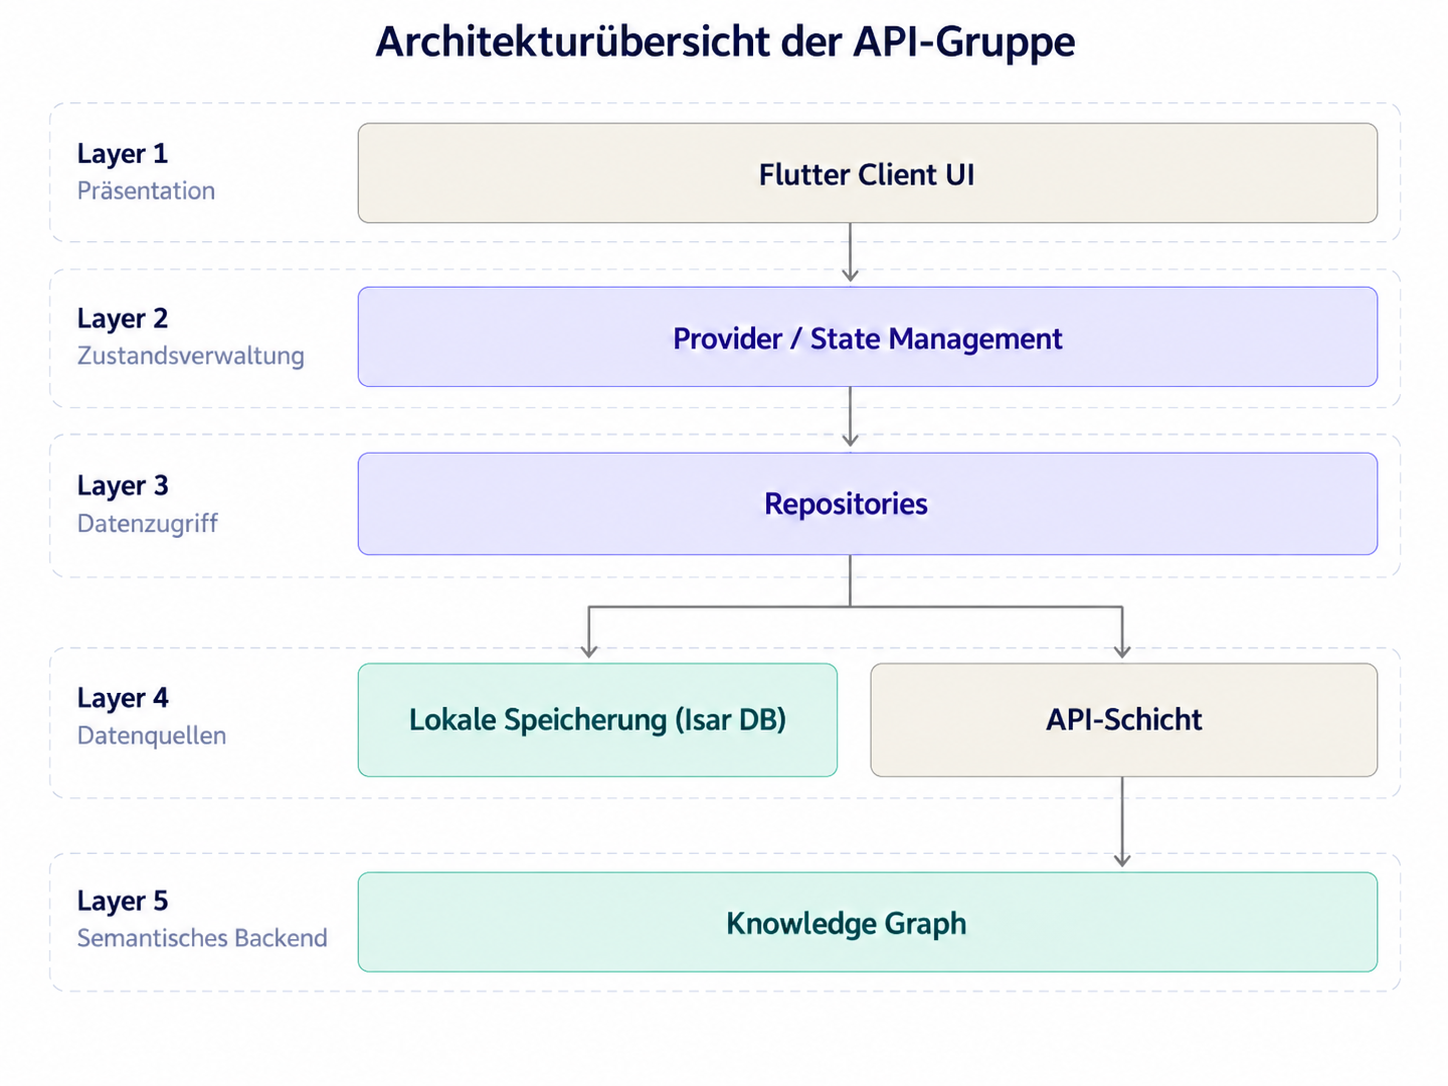
\includegraphics[width=0.8\textwidth]{bilder/API_1.png}
    \caption{Architekturdiagramm der Anwendung}
    \label{fig:architektur}
\end{figure}

\subsubsection{Lokale Entwicklungsumgebung und System-Setup}

Für die gemeinsame Entwicklung und das Testen der verschiedenen Komponenten wurde eine lokale Entwicklungsumgebung eingerichtet. Diese umfasste die Flutter-Anwendung, den Emulator, die lokale Isar-Datenbank sowie den Apache Jena Fuseki Server. Änderungen an der Ontologie wurden dabei regelmäßig mit der API abgestimmt, um die SPARQL-Abfragen entsprechend anzupassen. Für wiederkehrende Entwicklungsbefehle, wie die Code-Generierung oder die Konvertierung der Ontologie für den Knowledge Graph, wurde zudem Derry eingesetzt. Dadurch konnte ein stabiles technisches Fundament für die anwendungsübergreifende Zusammenarbeit geschaffen werden.

Für die lokale Ausführung des Projekts wurde ein ausführlicher Setup-Guide verfasst, der eine Schritt-für-Schritt-Anleitung zur Einrichtung aller dafür erforderlichen Komponenten enthält.

\paragraph{Testen der App}

Während der Entwicklung konnte die App sowohl auf einem mobilen Emulator als auch als Client-Anwendung auf einem Desktop-PC ausgeführt werden, wodurch die Benutzeroberfläche und der Zugriff auf die Daten gleichzeitig geprüft werden konnten. Ein wesentlicher Schwerpunkt lag dabei auf der Kontrolle, ob Daten in der Isar-Datenbank korrekt gespeichert, verändert und wieder geladen werden. Dadurch konnten Schnittstellenfehler und Probleme bei der Datenverarbeitung frühzeitig erkannt und behoben werden.


\subsection{Entwicklung}
\subsubsection{Architektur und Implementierung der SPARQL-API}
\label{sec:api-sparql}
\paragraph{Konzeptioneller Aufbau der API-Architektur}

Bereits in der Designphase -- im Anschluss an die Auswertung der User-Study -- zeichnete sich ab, dass der Knowledge Graph Daten für mehrere Anwendungsfunktionen (Features) über unterschiedliche SPARQL-Abfragen bereitstellen muss. Dies hatte konzeptionelle Auswirkungen auf die Gestaltung der API-Architektur im Flutter-Projekt.

Um im Quellcode Redundanzen zu vermeiden und das Trennungsprinzip (Separation of Concerns) einzuhalten, wurden alle featurerelevanten Request-Funktionen in eigene API-Klassen gekapselt. Diese Klassen enthalten lediglich die für das jeweilige Feature spezifische SPARQL-Abfrage, die zur Laufzeit dynamisch parametrisiert wird. Die eigentliche Logik für die HTTP-Kommunikation wurde vollständig in eine generische Kernklasse ausgelagert. Dort ist der gesamte Quellcode gebündelt, der für das Abschicken und Empfangen der SPARQL-Anfragen über HTTP verantwortlich ist.

Diese Zentralisierung ist möglich, da im vorliegenden Anwendungsfall alle Anfragen an den Apache-Fuseki-Server ausschließlich lesend erfolgen. Jede Anfrage wird als POST-Request mit identischen HTTP-Headern übertragen, um den Server über die Art des Inhalts sowie das erwartete Antwortformat zu informieren:

\begin{lstlisting}[caption={HTTP-Header der SPARQL-Anfragen}, label={lst:http_header}]
Content-Type: application/sparql-query
Accept: application/sparql-results+json
\end{lstlisting}

Im Request-Body wird stets ein SPARQL-String übermittelt; als Response liefert der Server ein SPARQL-JSON-Objekt zurück. Alle feature-spezifischen API-Klassen nutzen diesen generischen Rahmen, wodurch Code-Duplizierung vermieden wird. Die API-Klassen selbst werden bei Bedarf von den entsprechenden Repository-Klassen der Anwendung aufgerufen.

\begin{lstlisting}[caption={Aufrufkette einer SPARQL-Anfrage}, label={lst:aufrufkette}]
[Repository] --> [Feature-API-Klasse] --(SPARQL-Query)--> [Generische HTTP-Kernklasse] --(POST)--> [Apache Fuseki]
\end{lstlisting}

\paragraph{Workflow zur SPARQL-Entwicklung, Testen und Ontologie-Iteration}

Die Formulierung der SPARQL-Queries konnte weitgehend unabhängig vom Flutter-Projekt erfolgen. Dies bot dem Team die Möglichkeit, Kenntnisse im Verfassen von SPARQL-Abfragen auf Basis des Knowledge-Graphs aufzubauen.

Anfänglich wurde versucht, Queries direkt über die Konsole in Protégé zu entwickeln. Dieser Ansatz erwies sich jedoch aus zwei Gründen als unpraktikabel für den Entwicklungs- und Testprozess:
\begin{enumerate}
    \item Das Zurücksetzen von Änderungen war innerhalb der Umgebung nicht verlässlich möglich.
    \item Es fehlte eine native Unterstützung für Syntax-Highlighting; externe Plugins ließen sich nicht stabil einbinden.
\end{enumerate}

Als Lösung wurde auf die Webanwendung des Apache-Fuseki-Servers zurückgegriffen, die eine integrierte Query-Konsole mit Syntax-Highlighting bietet. Zudem stellt Fuseki die Ergebnisse sowohl in Tabellenform als auch im JSON-Format bereit, was die spätere Weiterverarbeitung in der Flutter-App widerspiegelt. Ein organisatorischer Aufwand bestand darin, bei Änderungen der Ontologie die aktuellste Version neu zu bauen und den Fuseki-Server anschließend neu zu starten. Dieser Prozess wurde im weiteren Verlauf über den Derry Script Manager teils automatisiert.

Eine zentrale Herausforderung lag in der parallelen Weiterentwicklung der Ontologie durch das Knowledge-Graph-Team. Für die API-Gruppe war es daher essenziell, die Struktur der Ontologie im Detail zu kennen, um Anpassungen zeitnah in den Queries nachzuziehen. Zur visuellen Inspektion der Ontologie-Struktur kam Protégé zum Einsatz. Durch die einfache Modellierung konnten die benötigten Instanzen rasch über entsprechende Object Properties und Data Properties gefiltert werden. Ein enger und kontinuierlicher Austausch mit der Knowledge-Gruppe stellte sicher, dass Schemaänderungen direkt berücksichtigt wurden.

Das Testen und Debuggen der Ergebnisse erfolgte manuell in der Fuseki-Weboberfläche: Einzelne Instanzen aus der Ontologie wurden als Stichproben ausgewählt und überprüft, ob sie unter den definierten SPARQL-Kriterien in der Ergebnismenge auftauchten. Angesichts des gegebenen Datenumfangs war diese manuelle Verifikation vertretbar.

Nach erfolgreicher Validierung wurden die Abfragen als Strings in die jeweiligen API-Klassen übernommen. Dynamische Variablen (\texttt{VALUES}) werden zur Laufzeit mittels String-Interpolation über App-Parameter und Nutzerprofil-Daten in das Query-Property eingesetzt, um die Ergebnismenge nutzerspezifisch zu filtern.

\paragraph{Implementierte API-Klassen}

Im Projekt wurden API-Klassen und SPARQL-Queries für die folgenden vier Hauptfeatures umgesetzt:
\begin{itemize}
    \item \textbf{Planerstellung} (\texttt{ExerciseAPI})
    \item \textbf{Planempfehlung} (\texttt{ExerciseAPI})
    \item \textbf{Rezept der Woche} (\texttt{RecipeAPI})
    \item \textbf{Tagestipps} (\texttt{DailyLifeAdviceAPI})
\end{itemize}

\subparagraph{Detaillierte Betrachtung: Die Klasse \texttt{ExerciseAPI} (Planerstellung und Planempfehlung)}

Die für die \textit{Planerstellung} und \textit{Planempfehlung} benötigten Daten werden über die API-Klasse \texttt{ExerciseAPI} abgefragt, welche jeweils eine dedizierte Methode für beide Anwendungsfälle bereitstellt. Beide Features nutzen ein analog aufgebautes SPARQL-Query. Nachfolgend wird der Aufbau der Abfrage anhand der im Query nummerierten Abschnitte im Detail erläutert (vgl. Listing~\ref{lst:sparql_exercise}):

\begin{enumerate}
    \item \textbf{\texttt{SELECT}-Klausel und Aggregation (Abschnitte 1 und 1.1):}
    Aus der Ontologie werden gezielt diejenigen Annotationen, Data Properties und Object Properties selektiert, die im Projektteam für die Weiterverarbeitung vereinbart wurden. Properties mit eineindeutigen Werten werden direkt übernommen. Für Eigenschaften, die nach einer Gruppierung mehrere Werte annehmen können (z.\,B. Kontraindikationen), kommt \texttt{GROUP\_CONCAT} zum Einsatz. Die Werte werden dabei mit dem Trennzeichen \texttt{|} in einem einzelnen String zusammengefasst (Abschnitt 1.1). Dies vereinfacht das spätere Parsing und Mappen in Dart-Listen innerhalb der App erheblich.

    \item \textbf{Dynamische Parameter-Einschränkung (\texttt{WHERE}-Block und \texttt{VALUES}, Abschnitte 2 bis 2.3.1):}
    Der \texttt{WHERE}-Block enthält die Kernlogik zur Verknüpfung und Filterung. Über \texttt{VALUES}-Blöcke werden die von der App übergebenen Benutzerparameter injiziert:
    \begin{itemize}
        \item \textbf{Trainingslevel (2.1):} Legt den Schwierigkeitsgrad fest (z.\,B. \textit{Beginner}, \textit{Intermediate}, \textit{Advanced}). Höhere Level schließen niedrigere Stufen logisch mit ein.
        \item \textbf{Trainingseffekt / Ziel (2.2):} Filtert nach spezifischen Zielen (\textit{Mobility}, \textit{Strength} etc.). Dieser Parameter ist optional (Mehrfachauswahl); wird kein Ziel übergeben, entfällt die Einschränkung.
        \item \textbf{Körperbereich (2.3 und 2.3.1):} Beschränkt die Abfrage auf ausgewählte Körperregionen (Einfachauswahl). Mittels Typenprüfung (2.3.1) werden ausschließlich Instanzen der Klassen \texttt{BodyPart} oder der Subklasse \texttt{Muscle} zugelassen. Dies verhindert fehlerhafte Ergebnisse durch Instanzen der Subklasse \texttt{Joint}, die an anderer Stelle verwendet werden.
    \end{itemize}

    \item \textbf{Obligatorische Object Properties (3):}
    Bestimmt, welche Beziehungen zwingend vorhanden sein müssen (z.\,B. zugewiesenes Schwierigkeitslevel, betroffener Körperbereich, erzielbarer Trainingseffekt). Übungen, denen diese Kernmetadaten fehlen, werden direkt ausgeschlossen, da sie in der Benutzeroberfläche nicht vollständig dargestellt werden könnten.

    \item \textbf{Ausschluss über Gelenke / Kontraindikationen (\texttt{FILTER NOT EXISTS}, Abschnitte 4 und 5):}
    \begin{itemize}
        \item \textbf{Gelenk-Filter (4):} Schließt Übungen aus, die mit medizinischen Einschränkungen an spezifischen Gelenken (\textit{Joints}) kollidieren (z.\,B. Ausschluss von Liegestützen bei Ellenbogenproblemen).
        \item \textbf{Soft-Filter für Kontraindikationen (5):} Entfernt Übungen bei allgemeinen Beschwerden (z.\,B. Hüft- oder Rumpfprobleme). Hier greift jedoch eine \textbf{Ausnahmeregel}: Gehört eine Übung zu den Subklassen \texttt{Mobilisation}, \texttt{Relaxation} oder \texttt{Stretching}, wird sie durch diesen Kontraindikationsfilter \textit{nicht} ausgeschlossen. Diese Ausnahme entspricht der implementierten Abfragelogik und stellt keine medizinische Freigabe dar. Der separate Gelenk-Filter bleibt davon unberührt.
    \end{itemize}

    \item \textbf{Labels und Basiseigenschaften (6):}
    Stellt sicher, dass für die verbleibenden Instanzen die Klartext-Labels (\texttt{rdfs:label}) für Kontraindikationen, Effekte und Körperbereiche geladen werden. Zudem wird das Vorhandensein zwingender Data Properties (\texttt{hasInstruction}, \texttt{hasDuration}) geprüft.

    \item \textbf{Fallback-Logik für Beschreibungen (7):}
    Beschreibungen befinden sich daher entweder in der Property \texttt{hasDescription} oder der Annotation \texttt{rdfs:comment}. Mittels \texttt{OPTIONAL} und \texttt{BIND(COALESCE(...))} wird bevorzugt \texttt{hasDescription} ausgewertet; existiert diese nicht, wird auf \texttt{rdfs:comment} zurückgegriffen. Besitzt eine Übung weder das eine noch das andere, wird sie über \texttt{FILTER(BOUND(?description))} aus der Ergebnismenge entfernt.

    \item \textbf{Sprachfilterung (8):}
    Die Ontologie führt stellenweise mehrsprachige Labels (\texttt{DE} und \texttt{EN}). Da die App-Implementierung auf Deutsch fokussiert wurde, erzwingt ein \texttt{FILTER} die Rückgabe deutscher Texte für Übungstitel und Beschreibungen, um Duplikate im Resultat zu vermeiden.

    \item \textbf{Optionale Zusatzmedien und Formatter (9 und 10):}
    Zusätzliche Hilfen wie Ausführungsfehler (\texttt{hasCommonMistake}), Korrekturhinweise (\texttt{hasCorrectionGuidance}), Bild- und Video-URLs werden optional geladen (9). Zudem wird die URI des Schwierigkeitsgrades via Regex-Operation (\texttt{REPLACE}) in ein lesbares String-Label transformiert (10).

    \item \textbf{Gruppierung (11):}
    Der abschließende \texttt{GROUP BY}-Befehl verdichtet alle Multi-Value-Eigenschaften pro Übung, sodass der Fuseki-Server exakt ein eindeutiges JSON-Objekt pro Übung an die Flutter-Anwendung zurücksendet.
\end{enumerate}

\begin{lstlisting}[caption={SPARQL-Query der Klasse \texttt{ExerciseAPI} für Planerstellung und Planempfehlung}, label={lst:sparql_exercise}]
PREFIX re: <http://www.w3.org/2000/10/swap/reason#>
PREFIX owl: <http://www.w3.org/2002/07/owl#>
PREFIX rdf: <http://www.w3.org/1999/02/22-rdf-syntax-ns#>
PREFIX rdfs: <http://www.w3.org/2000/01/rdf-schema#>
PREFIX rehab: <http://purl.org/PhysicalTherapy#>

# 1. Selektiert gefilterte Übungen mit entsprechenden Eigenschaften für die Planerstellung und -empfehlung
SELECT
    ?exercise
    ?exerciseLabel
    ?description
    ?difficultyLabel
    ?duration
    ?instruction
    ?video
    ?pic
    # 1.1 Verpackt alle Values der Gruppe in einem Value String mit Trennzeichen
    (GROUP_CONCAT(DISTINCT ?contraindicationLabel; separator=" | ") AS ?contraindications)
    (GROUP_CONCAT(DISTINCT ?trainingsEffectLabel; separator=" | ") AS ?trainingsEffects)
    (GROUP_CONCAT(DISTINCT ?bodyPartLabel; separator=" | ") AS ?bodyParts)
    (GROUP_CONCAT(DISTINCT ?correction; separator=" | ") AS ?corrections)
    (GROUP_CONCAT(DISTINCT ?mistake; separator=" | ") AS ?mistakes)
WHERE {
    # 2. Filterparameter (werden zur Laufzeit übergeben)
    # 2.1 Trainingslevel
    VALUES ?difficulty {
        rehab:Beginner
        rehab:Intermediate
        rehab:Advanced
    }

    # 2.2 Gewünschte Trainingseffekte
    VALUES ?trainingsEffect {
        rehab:Balance
        rehab:Coordination
        rehab:Flexibility
        rehab:Focus
        rehab:Mobility
        rehab:Posture
        rehab:Relaxation
        rehab:Stability
        rehab:Strength
    }

    # 2.3 Gewünschte Körperbereiche (Enthält nun BodyPart- UND Muscle-Instanzen)
    VALUES ?bodyPart {
        # --- BodyPart Instanzen ---
        rehab:Ankles rehab:Arms rehab:Back rehab:Bauch rehab:Calves rehab:Chest rehab:Core rehab:Elbows
        rehab:Glutes rehab:Hip rehab:Knees rehab:Legs rehab:LowerBack rehab:Neck rehab:Pelvic
        rehab:Shoulders rehab:Spine rehab:Thighs rehab:UpperBack rehab:Wrists

        # --- Muscle Instanzen ---
        rehab:Abs rehab:Adductors rehab:Biceps rehab:ForearmFlexors rehab:FrontDeltoid
        rehab:Hamstrings rehab:LateralDeltoids rehab:Lats rehab:Obliques rehab:Quadriceps
        rehab:Quads rehab:RearDeltoids rehab:RotatorCuffs rehab:Shoulder rehab:Trapezius rehab:Triceps
    }

    # 2.3.1 Exakte Typenprüfung: Nur direkte BodyPart- ODER Muscle-Instanzen zulassen
    ?bodyPart a ?bodyPartType .
    FILTER(?bodyPartType IN (rehab:BodyPart, rehab:Muscle))

    # 3. Übungen müssen alle benötigten Object Properties besitzen
    ?exercise a/rdfs:subClassOf* rehab:Exercise ;
              rehab:hasDifficultyLevel ?difficulty ;
              rehab:hasContraindication ?contraindication ;
              rehab:improves ?trainingsEffect ;
              rehab:engagedBodyPart ?bodyPart .

    ?contraindication a rehab:Contraindication .
    ?trainingsEffect a rehab:TrainingsEffect .

    # 4. Entfernt Übungen, die mit betroffenen Gelenken (Joints) kollidieren
    FILTER NOT EXISTS {
        VALUES ?selectedJoints {
            # rehab:HipJoint
            # rehab:ShoulderJoint
        }
        # Stellt sicher, dass das ausgewählte Element ein Joint ist (Subclass von BodyPart)
        ?selectedJoints a/rdfs:subClassOf* rehab:Joint .
        ?exercise rehab:engagedBodyPart ?selectedJoints .
    }

    # 5. Entfernt Übungen mit angegebenen Contraindications,
    # AUSSER die Übung stammt von den Klassen Mobilisation, Relaxation oder Stretching ab.
    FILTER NOT EXISTS {
        VALUES ?selectedContraindication {
            # rehab:HipIssue
            # rehab:ShoulderIssue
        }
        ?exercise rehab:hasContraindication ?selectedContraindication .

        # Ausnahmeregel: Wenn die Übung vom Typ (oder einer Subklasse von)
        # Mobilisation, Relaxation oder Stretching ist, greift der Ausschluss NICHT.
        FILTER NOT EXISTS {
            VALUES ?exceptionClass {
                rehab:Mobilisation
                rehab:Relaxation
                rehab:Stretching
            }
            ?exercise a/rdfs:subClassOf* ?exceptionClass .
        }
    }

    # 6. Übungen müssen diese Labels und Eigenschaften besitzen
    ?contraindication rdfs:label ?contraindicationLabel .
    ?trainingsEffect rdfs:label ?trainingsEffectLabel .
    ?bodyPart rdfs:label ?bodyPartLabel .
    ?exercise rehab:hasInstruction ?instruction ;
              rehab:hasDuration ?duration ;
              rdfs:label ?exerciseLabel .

    # 7. Beschreibung ermitteln: hasDescription bevorzugen, rdfs:comment als Fallback
    OPTIONAL { ?exercise rehab:hasDescription ?hasDesc }
    OPTIONAL {
        ?exercise rdfs:comment ?rdfsComment .
        FILTER(LANG(?rdfsComment) = "" || LANGMATCHES(LANG(?rdfsComment), "de"))
    }
    BIND(COALESCE(?hasDesc, ?rdfsComment) AS ?description)

    # Wenn weder hasDescription noch rdfs:comment existiert -> Übung ausschließen
    FILTER(BOUND(?description))

    # 8. Labels sind mehrsprachig und werden auf die notwendige Sprache für die Datenverarbeitung beschränkt
    FILTER(
        LANGMATCHES(LANG(?contraindicationLabel), "en") &&
        LANGMATCHES(LANG(?trainingsEffectLabel), "en") &&
        LANGMATCHES(LANG(?bodyPartLabel), "en") &&
        LANGMATCHES(LANG(?exerciseLabel), "de") &&
        (LANG(?description) = "" || LANGMATCHES(LANG(?description), "de"))
    )

    # 9. Optionale Zusatzinformationen
    OPTIONAL { ?exercise rehab:hasCorrectionGuidance ?correction }
    OPTIONAL { ?exercise rehab:hasCommonMistake ?mistake }
    OPTIONAL { ?exercise rehab:hasVideoUrl ?video }
    OPTIONAL { ?exercise rehab:hasPicUrl ?pic }

    # 10. Extrahiert den lokalen Namen der Difficulty-URI
    BIND(REPLACE(STR(?difficulty), "^.*[#/]", "") AS ?difficultyLabel)
}
# 11. Gruppierung
GROUP BY
    ?exercise
    ?exerciseLabel
    ?description
    ?difficultyLabel
    ?duration
    ?instruction
    ?video
    ?pic
\end{lstlisting}

\subparagraph{\texttt{RecipeAPI} (\textit{Rezept der Woche})}
Beim Start einer neuen Trainingswoche können Nutzer:innen -- abhängig vom Erreichen eines Wochen-Streaks -- ein neues Rezept freischalten. Die Klasse \texttt{RecipeAPI} fragt alle Rezepte aus dem Knowledge Graph ab, die von den Nutzer:innen noch nicht freigeschaltet wurden. Die ID-Liste der bereits freigeschalteten Rezepte wird dabei als Filterparameter im SPARQL-Query übergeben.

\subparagraph{\texttt{DailyLifeAdviceAPI} (\textit{Tagestipps})}
Diese Klasse ruft passend zu den aktuell von den Nutzer:innen trainierten Körperregionen Kontext-Tipps für den Alltag ab. Die SPARQL-Abfrage filtert die Tipps basierend auf den primär adressierten Muskelgruppen bzw. Körperbereichen.

\medskip
\noindent\textbf{Dokumentationshinweis:} Alle in der Produktionsumgebung eingesetzten SPARQL-Queries wurden in einem separaten Markdown-Dokument fortlaufend strukturiert, kommentiert und versioniert.


\subsubsection{Verarbeitung der API-Daten}

Die Daten aus dem Knowledge Graph kommen vom Fuseki-Server als SPARQL-JSON zurück. Mit diesem Format kann die App selbst noch nicht direkt arbeiten. Deshalb werden die Antworten nach dem Abruf zuerst in passende Formate transformiert und anschließend in Dart-Modelle geparst, aus denen die entsprechenden Objekte mit den Daten konstruiert werden.

Dabei war vor allem zu berücksichtigen, dass einige Eigenschaften einer Übung mehrere Werte haben können. Eine Übung kann etwa mehreren Körperbereichen zugeordnet sein oder mehrere Trainingseffekte, Korrekturhinweise und typische Fehler besitzen. Diese Werte werden in der SPARQL-Abfrage, wie bereits erwähnt, in Form von String-Properties zusammengefasst übertragen. In der App werden sie anschließend über vordefinierte Mapper-Funktionen wieder aufgeteilt und als Listen in den entsprechenden Dart-Modellen gespeichert.

Dabei erhält nicht jede Property dieselbe Mapper-Funktion. Betrachtet man die Eigenschaft der Übungsanweisungen, zeigt sich, dass in der Ontologie die einzelnen Schritte nicht als getrennte Felder vorliegen, sondern als ein gemeinsamer Text mit nummerierten Abschnitten. Nach dem Abruf zerlegt die Mapper-Funktion den Inhalt anhand dieser Nummerierung in einzelne Schritte. Dadurch kann die UI die Anleitung später Schritt für Schritt darstellen, indem die Reihenfolge der Liste berücksichtigt wird.

Nicht alle geladenen API-Daten werden gleich behandelt. Die Übungsdaten werden während der Nutzung zunächst im Arbeitsspeicher gehalten und stehen dort für die Auswahl bei der Planerstellung zur Verfügung. Erst wenn ein Plan mit den entsprechenden Übungen erstellt wurde, werden diese auch in Isar persistent gespeichert.

Bei den Schonungstipps für den Alltag verhält es sich hingegen anders: Diese Daten werden vom Knowledge Graph abgerufen und direkt an die UI weitergeleitet. Für sie besteht keine Notwendigkeit einer lokalen Speicherung, da die Ergebnismenge lediglich vom Filter für die aktiv trainierten Körperbereiche abhängt.

\subsubsection{Repositories und Provider}
\label{sec:api-repos}

Für den Zugriff auf die Daten werden Repositories und Provider verwendet. Die Repositories kümmern sich darum, woher die Daten kommen und wo sie gespeichert werden. Das kann die lokale Isar-Datenbank sein oder die API zum Knowledge Graph. Die Provider verwenden diese Repositories und halten die Daten, die gerade in der App benötigt werden, im Arbeitsspeicher. Wenn sich dort etwas ändert, wird die UI darüber informiert und kann sich entsprechend aktualisieren.

Ein wichtiger Punkt ist der Schmerzverlauf. Die eingetragenen Schmerzwerte werden nicht nur einzeln im Graphen dargestellt, sondern es soll zusätzlich erkannt werden, ob sich der Verlauf über einen Monat eher verbessert oder verschlechtert. Dafür wird eine lineare Regression über die vorhandenen Einträge verwendet. Aus den Messwerten wird eine Trendlinie berechnet und die Veränderung auf einen Zeitraum von 30 Tagen übertragen. Für die Berechnung müssen mindestens drei Einträge vorhanden sein. Erst ab einer Veränderung von 0,8 wird ein steigender oder fallender Trend angezeigt. Die Grenze von 0,8 ist der im Prototyp verwendete Schwellenwert für die Anzeige eines Trends. Kleinere rechnerische Veränderungen lösen keinen Trendhinweis aus; die Anzeige stellt keine medizinische Beurteilung des Schmerzverlaufs dar. Der Trend selbst wird nicht gespeichert, sondern stets aus den vorhandenen Einträgen neu berechnet.

Eine weitere Logik betrifft den Weekly Streak. Dafür werden die gespeicherten Trainingseinträge nach Kalenderwoche und Trainingsplan ausgewertet. Eine Woche zählt als erfolgreich, wenn für mindestens einen aktiven Plan die vorgesehene Anzahl an Trainingseinheiten erreicht wurde. Anschließend wird geprüft, wie viele erfolgreiche Wochen direkt aufeinanderfolgen. Für die aktuelle Woche gibt es dabei einen Sonderfall: Sie muss noch nicht abgeschlossen sein, damit ein bereits vorhandener Streak bestehen bleibt. Andernfalls würde eine Person ihren Streak direkt am Anfang einer neuen Woche verlieren, obwohl sie noch gar keine Möglichkeit hatte, alle geplanten Einheiten durchzuführen.

Die Weekly Streak wird außerdem für die Freischaltung von Rezepten verwendet. Steigt die Streak und wurde für diesen Fortschritt noch kein Rezept vergeben, werden zunächst die bereits freigeschalteten Rezepte ermittelt. Diese IDs werden bei der Abfrage des Knowledge Graphs ausgeschlossen. Aus den übrigen Rezepten wird zufällig eines ausgewählt und anschließend mit dem Zeitpunkt der Freischaltung in Isar gespeichert. Zusätzlich wird festgehalten, ob ein bestimmter Streak bereits verarbeitet wurde. Dadurch wird verhindert, dass dieselbe Änderung mehrfach eine Rezeptfreischaltung auslöst. Bei diesem Ablauf greifen lokale Daten und der Knowledge Graph direkt ineinander: Der Trainingsfortschritt stammt aus den gespeicherten Logs, das neue Rezept kommt aus dem Knowledge Graph und das freigeschaltete Ergebnis wird anschließend wieder lokal gespeichert.

Ein weiterer Bereich ist die Auswertung der Trainingszustände während des Workouts. Wenn eine Person eine Übung absolviert, speichert das Repository diesen Eintrag mit der zugehörigen Plan-ID und einem Zeitstempel in der lokalen Isar-Datenbank. Der Provider lädt diese Einträge in den Arbeitsspeicher und berechnet daraus die Zustände für die Benutzeroberfläche. Über einen Abgleich der heutigen Logs mit den Übungen des Plans wird der aktuelle Tagesfortschritt ermittelt, der beispielsweise im Plan-Detailbildschirm als Fortschrittsbalken angezeigt wird. Im eigentlichen Trainingsflow übernimmt der Provider zudem die Ablaufsteuerung: Er prüft vorab, ob die aktuell geöffnete Übung die letzte noch fehlende des Plans ist. Dadurch kann die UI die Beschriftung des Buttons dynamisch von \glqq Nächste Übung\grqq{} auf \glqq Training abschließen\grqq{} anpassen und direkt die passende Abschlussaktion auslösen. Wird ein unterbrochenes Training später erneut geöffnet, ermittelt der Provider automatisch den Index der ersten noch offenen Übung, sodass an der richtigen Stelle weitergetrainiert werden kann. Wird festgestellt, dass eine Trainingseinheit für den heutigen Tag abgeschlossen ist, teilt der Provider dies der UI mit, damit der entsprechende Button zum Starten des Trainings für heute deaktiviert wird.

\subsubsection{Datenfluss bis zur UI}

Zur Veranschaulichung des gesamten Datenflusses bietet es sich an, das Laden der Übungen für die Planerstellung genauer zu betrachten. Nutzer:innen wählen in der Oberfläche eine Körperregion und ein Trainingsziel aus. Diese Auswahl wird über den Provider an das Repository weitergegeben. Dort werden die im Nutzerprofil hinterlegten Angaben zu betroffenen Gelenken, Kontraindikationen und Trainingslevel berücksichtigt.

Diese Angaben sind die Vorlage für den Aufbau der Parameter für die SPARQL-Abfrage. Die Anfrage wird über die API an den Fuseki-Server geschickt, und der Knowledge Graph liefert die passenden Übungsdaten zurück. Danach wird die JSON-Antwort verarbeitet und in Dart-Objekte umgewandelt. Erst diese fertigen Objekte gehen wieder zurück an den Provider.

Der Provider übernimmt die neue Übungsliste in seinen aktuellen Zustand und informiert die Benutzeroberfläche über die Änderung. Die UI muss dabei nicht wissen, wie die SPARQL-Abfrage aufgebaut ist oder wie die Serverantwort verarbeitet wurde. Sie erhält am Ende nur die bereits aufbereiteten Übungen.

Bei lokalen Daten ist der Ablauf ähnlich. Trägt eine Person einen neuen Schmerzwert ein, nimmt zunächst der Provider die Eingabe entgegen und gibt sie an das Repository weiter. Dort wird geprüft, ob für dieselbe Körperregion und denselben Tag bereits ein Eintrag vorhanden ist. Danach wird der Eintrag in Isar gespeichert und die aktuelle Liste der Schmerzdaten erneut geladen. Der Provider übernimmt anschließend diesen neuen Stand. Für die Anzeige des Schmerzverlaufs können die Einträge nach Monat und Körperregion gefiltert und für den Graphen verwendet werden. Der Trend wird auf Grundlage dieser Werte berechnet und muss deshalb nicht zusätzlich in der Datenbank gespeichert werden.

Auch die Rezeptfreischaltung nutzt beide Datenquellen: Nach abgeschlossenen Trainingseinheiten werden die Trainingsdaten zunächst lokal gespeichert und der Weekly Streak neu berechnet. Ergibt sich daraus eine neue Freischaltung, werden noch nicht freigeschaltete Rezepte über die API aus dem Knowledge Graph geladen. Eines davon wird zufällig ausgewählt, lokal gespeichert und danach über den Provider für die UI bereitgestellt.

Auf diese Weise arbeitet die Benutzeroberfläche nicht direkt mit Isar oder Fuseki. Der Zugriff auf die Daten und die dazugehörige Verarbeitung bleiben vollständig in den darunterliegenden Schichten gekapselt.


\subsection{Lokale Datenspeicherung}
\subsubsection{Motivation und Entwurfsentscheidungen}
\label{sec:api-isar-motivation}

Die App begleitet Nutzer:innen über mehrere Wochen durch ein Trainingsprogramm, und dabei entstehen zwei Arten von Daten. Die erste sind Inhalte wie Übungen, Alltagstipps und Rezepte. Sie liegen im Knowledge-Graph und werden über die API geladen, wobei die Übungsauswahl anhand von Kontraindikationen, betroffenen Gelenken, Körperregionen und Trainingszielen gefiltert wird. Die zweite sind persönliche Daten: das Profil mit Alter, Gewicht, Körpergröße, Kontraindikationen, betroffenen Gelenken und Fitnesslevel, außerdem die zusammengestellten Trainingspläne, Schmerzprotokolle, Trainingslogs, der Wochenstatus und die freigeschalteten Rezepte. Diese zweite Gruppe muss dauerhaft auf dem Gerät gespeichert werden. Sie ist stark strukturiert und muss nach Datum, Körperregion und Status gefiltert werden können.

Es wurde sich bewusst gegen eine Cloud-Lösung mit Benutzerkonto entschieden. Eine Cloud hätte zwar geräteübergreifende Nutzung und Backups ermöglicht, aber Profil und Schmerzprotokolle enthalten gesundheitsbezogene Daten, wodurch zusätzliche datenschutzrechtliche Anforderungen entstehen können. Eine serverseitige Speicherung hätte Einwilligungsmanagement, Auftragsverarbeitung und zusätzliche Schutzmaßnahmen erfordert, was für das Projekt unverhältnismäßig wäre. Ein Login-Zwang würde außerdem die Einstiegshürde erhöhen, während die App ohne Registrierung sofort nutzbar sein soll. Die persönlichen Verlaufsdaten wie Pläne, Schmerzprotokolle und Trainingslogs werden ausschließlich lokal gespeichert, für sie wird keine serverseitige Datenbank verwendet, was dem Prinzip der Datenminimierung entspricht. Für die personalisierte Übungsauswahl werden allerdings die Kontraindikationen und betroffenen Gelenke als Filterparameter an die API übergeben. Der Preis der lokalen Speicherung ist, dass es keine Synchronisation zwischen Geräten gibt und die Daten bei Deinstallation oder Gerätewechsel verloren gehen. Diesen Kompromiss wurde bewusst in Kauf genommen.

Für eine Cloud-Variante wäre zusätzliche Infrastruktur notwendig gewesen. Zunächst müsste eine Möglichkeit geschaffen werden, Nutzerkonten zu verwalten und die persönlichen Daten eindeutig den jeweiligen Nutzern zuzuordnen. Zusätzlich müssten die persönlichen Daten auf einem Server gespeichert und über eine entsprechende Schnittstelle von der App abgerufen und verändert werden können. Wenn die App weiterhin offline funktionieren soll, wäre außerdem eine lokale Zwischenspeicherung sowie eine Synchronisation zwischen Gerät und Server notwendig. Dabei müsste auch berücksichtigt werden, wie mit Änderungen umgegangen wird, die während einer Offline-Nutzung entstehen.

Zusätzlich wären bei der Speicherung von persönlichen und gesundheitsbezogenen Daten weitere datenschutzrechtliche Anforderungen zu berücksichtigen. Dazu gehören unter anderem die sichere Speicherung und Übertragung der Daten sowie Möglichkeiten für die Nutzer:innen, ihre Daten einzusehen und löschen zu lassen. Auch für den laufenden Betrieb wären zusätzliche Aufgaben wie Hosting, Backups und Wartung notwendig. Eine lokale Datenbank wäre dabei auch in einer Cloud-Variante weiterhin sinnvoll, um die Daten offline verfügbar zu machen. Die jetzige Lösung bildet daher eine mögliche Grundlage für eine spätere Erweiterung um eine Synchronisation mit einem Server.

Für die lokale Speicherung kamen neben Isar auch einfachere Lösungen wie SharedPreferences oder Hive infrage, sowie relationale Datenbanken wie SQLite. SharedPreferences ist ein simpler Speicher für kleine Einstellungen, wie ihn praktisch jede App nutzt, etwa für den Dark Mode oder die Sprache, eignet sich aber nicht für strukturierte Listen mit Datumsabfragen und Filtern, da weder Abfragen noch Indizes zur Verfügung stehen. Hive ist ähnlich einfach gehalten und bietet als reiner Key-Value-Speicher ebenfalls keine echten Abfragen, sodass Filter nach Datum oder Körperregion manuell im Arbeitsspeicher umgesetzt werden müssten. Eine relationale Datenbank wie SQLite wäre technisch möglich gewesen, hätte aber deutlich mehr Aufwand bedeutet: Das Datenmodell enthält verschachtelte Objekte, etwa Trainingspläne mit einer variablen Anzahl an Übungen, die in einer relationalen Struktur über zusätzliche Tabellen und Verknüpfungen abgebildet werden müssten, statt einfach als Ganzes gespeichert zu werden. Isar erlaubt es dagegen, die Dart-Objekte direkt in dieser verschachtelten Form zu speichern und trotzdem effizient nach Datum, Region oder Status zu filtern. Für das Datenmodell aus Plänen mit eingebetteten Übungen und zeitbasierten Logs passte Isar daher mit dem geringsten Aufwand am besten.

\subsubsection{Umsetzung}
\label{sec:api-isar-umsetzung}

Die Datenhaltung ist in drei Ebenen aufgeteilt. Modelle definieren, welche Daten gespeichert werden, Repositories kapseln die Isar-Abfragen und Schreibvorgänge, die in Transaktionen mit \texttt{isar.writeTxn()} ausgeführt werden, und Provider laden die Daten aus den Repositories, halten sie im Arbeitsspeicher und informieren die Oberfläche über Änderungen. Widgets greifen dadurch normalerweise nicht direkt auf Isar zu, und Datenbanklogik bleibt von der Darstellung getrennt. Die Datenbank wird beim Start in \texttt{main.dart} im Dokumentenverzeichnis der App geöffnet, dessen Pfad über \texttt{path\_provider} ermittelt wird, und registriert dabei sieben Collections. Die zugehörigen \texttt{.g.dart}-Dateien werden aus den Isar-Annotationen mit \texttt{build\_runner} erzeugt. Tabelle~\ref{tab:isar_collections} gibt einen Überblick über die Collections.

\begin{table}[H]
    \centering
    \begin{tabular}{lp{10.5cm}}
        \hline
        \textbf{Collection} & \textbf{Gespeicherte Daten} \\
        \hline
        \texttt{User} & Name, Geschlecht, Alter, Gewicht, Größe, Kontraindikationen, betroffene Gelenke, Fitnesslevel \\
        \texttt{Plan} & interne ID, fachliche Plan-ID, Name, Körperregion, Ziele, eingebettete Übungen, Einheiten pro Woche, abgeschlossene Einheiten (\texttt{completedSessions}), Herkunft, Archivstatus, Farbe \\
        \texttt{AppState} & Zeitpunkt des nächsten Wochenresets (\texttt{nextResetDate}) \\
        \texttt{PainLog} & Intensität, Körperregion, Notiz, Datum und Uhrzeit (\texttt{date}), Datumsschlüssel (YYYY-MM-DD) \\
        \texttt{PainLogExercise} & Intensität, Region, Datum und Uhrzeit (\texttt{date}), Datumsschlüssel, optionale Plan- und Übungs-ID \\
        \texttt{PlanLogExercise} & Plan-ID, Übungs-ID, Zeitpunkt der Durchführung (\texttt{timestamp}) \\
        \texttt{Recipe} & ID, Beschreibung, gesundheitlicher Nutzen, Zubereitungsdauer, Freischaltzeitpunkt \\
        \hline
    \end{tabular}
    \caption{Collections der lokalen Isar-Datenbank}
    \label{tab:isar_collections}
\end{table}

Übungen werden nicht als eigenständige Collection gespeichert. Werden sie einem Trainingsplan hinzugefügt, werden die zu diesem Zeitpunkt vorhandenen Übungsdaten als eingebettete Objekte innerhalb des Plans persistiert, das zugehörige \texttt{ExerciseSchema} ist daher ein Embedded-Schema innerhalb von \texttt{PlanSchema}. Änderungen im Knowledge Graph wirken sich deshalb nicht automatisch auf bereits gespeicherte Pläne aus. Rezepte nehmen eine Zwischenstellung ein: Die Rezeptdaten stammen aus der API. Welche Rezepte freigeschaltet wurden, wird jedoch lokal gespeichert.

Bei der Verwaltung des Trainingsfortschritts gibt es zwei Ebenen. Die historischen Trainingsdaten werden in \texttt{PlanLogExercise} gespeichert und dienen zur Berechnung von Tagesfortschritt, abgeschlossenen Plänen und Wochenstreaks, sodass sich auch vergangene Trainingstage jederzeit rekonstruieren lassen. Zusätzlich speichert \texttt{Plan} den Zähler \texttt{completedSessions}, der für die Wochenringe und die Begrenzung der Trainingseinheiten verwendet wird. Der Zähler wird beim Abschluss eines Trainings direkt erhöht, beim Wochenreset auf null gesetzt und nach bestimmten Änderungen an den Trainingslogs neu berechnet. Logs und Pläne werden außerdem nicht über Isar-Relationen, sondern über einfache String-IDs (\texttt{planId}, \texttt{exerciseId}) verknüpft. Nicht persistiert werden Alltagstipps und reine UI-Zustände wie der ausgewählte Tab.

\begin{figure}[htbp]
    \centering
    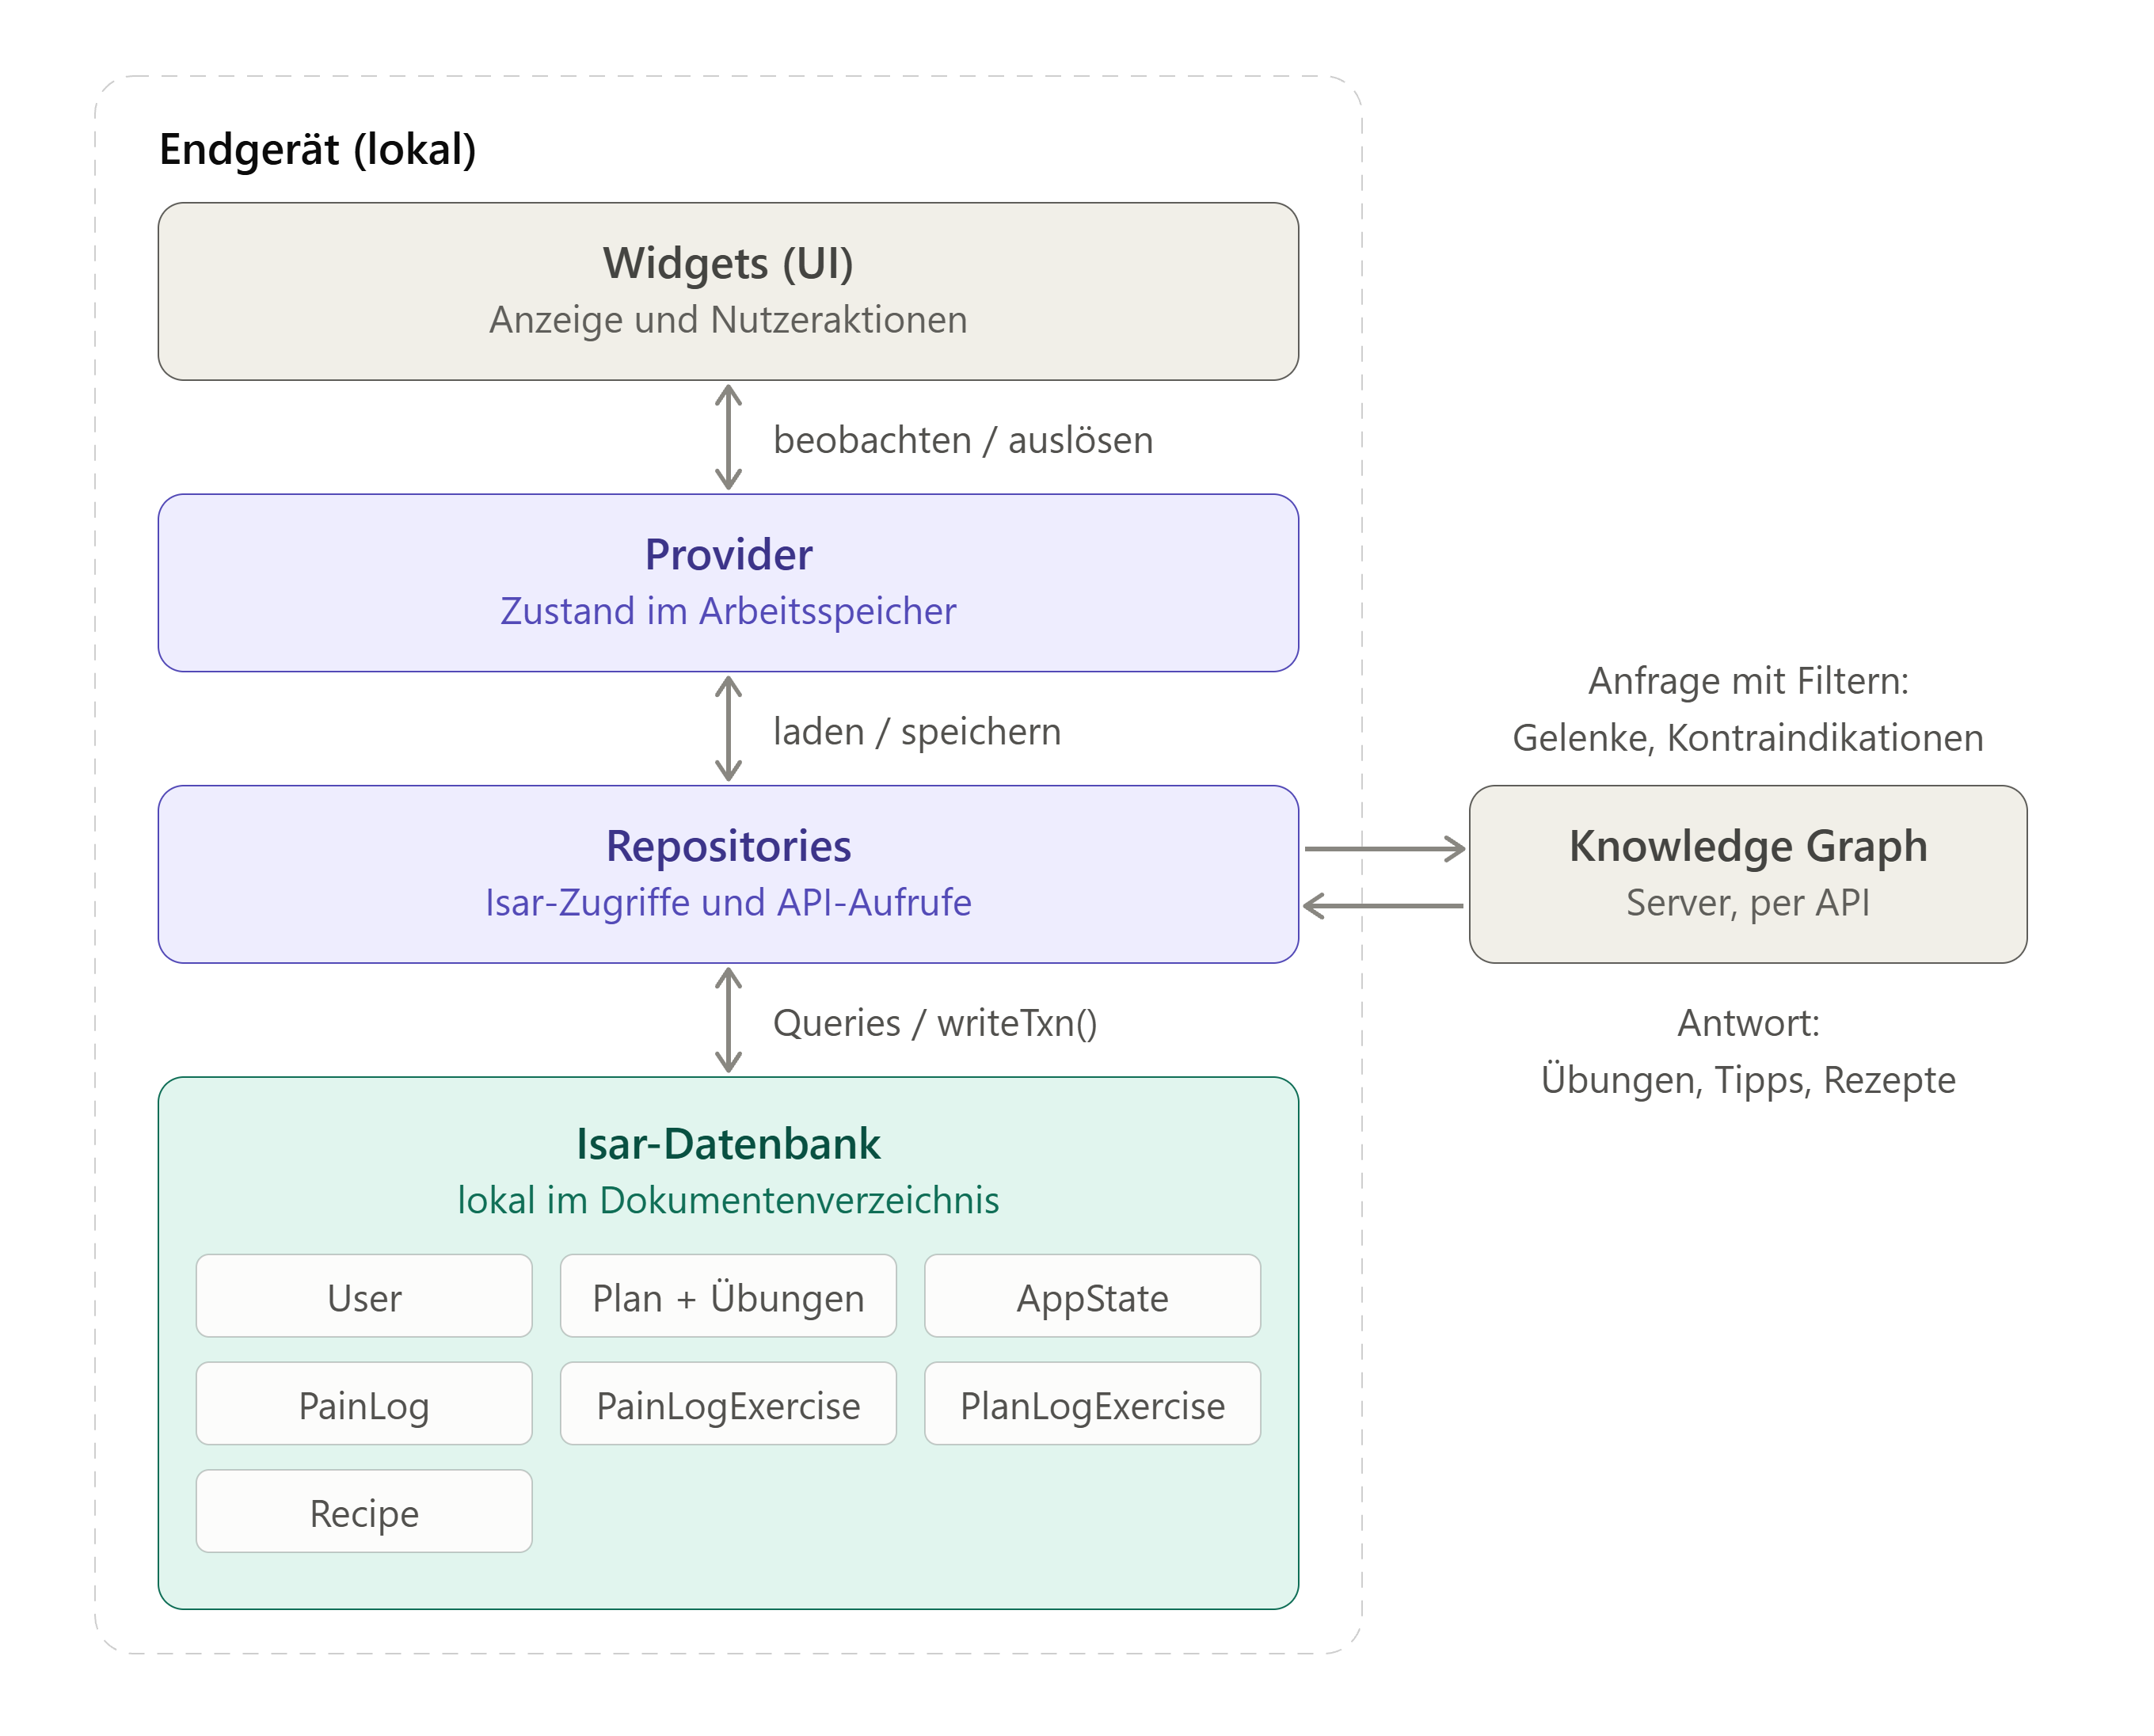
\includegraphics[width=0.8\textwidth]{bilder/API_2.png}
    \caption{Datenmodell der lokalen Isar-Datenbank}
    \label{fig:isar_datenmodell}
\end{figure}

\subsubsection{Herausforderungen}

Eine Einschränkung des Modells ist, dass Isar anders als eine klassische Datenbank keine feste Verknüpfung zwischen zusammengehörigen Daten erzwingt. Löscht man zum Beispiel einen Trainingsplan, werden die zugehörigen Trainingslogs nicht automatisch mitgelöscht. Dadurch können \glqq verwaiste\grqq{} Logs entstehen, die auf einen nicht mehr existierenden Plan verweisen. Bei der Berechnung des Fortschritts werden solche Logs einfach ignoriert, wenn der zugehörige Plan nicht mehr gefunden wird. Da Pläne meist archiviert statt endgültig gelöscht werden, tritt dieser Fall in der Praxis eher selten auf.

Eine weitere Herausforderung war das Gruppieren von Daten, also das Zusammenfassen einzelner Einträge zu Tages-, Monats- oder Regionswerten, etwa für den Kalender oder für Verlaufsgrafiken. Klassische Datenbanken können solche Gruppierungen direkt in einer Abfrage erledigen, Isar bietet diese Möglichkeit nicht. Das Gruppieren wird deshalb selbst im Code der App übernommen, nachdem die Daten geladen wurden. Damit das trotzdem schnell bleibt, sind die Felder für Datum und Körperregion in der Datenbank für schnellen Zugriff vorbereitet (indexiert), und für jeden Eintrag wird zusätzlich ein vereinfachter Tagesschlüssel gespeichert, der die Zuordnung zu einem bestimmten Tag erleichtert. Bei der überschaubaren Datenmenge, die pro Person und Tag anfällt, macht sich dieser zusätzliche Aufwand bei der Geschwindigkeit nicht bemerkbar.

Auch beim Bereich der Alltagstipps gibt es eine kleine Besonderheit: Die Tipps werden bei jedem Öffnen der App neu von der API geladen und nur vorübergehend im Arbeitsspeicher gehalten, eine dauerhafte Speicherung ist hier auch nicht vorgesehen. Für eine mögliche spätere Speicherung wurde zwar bereits ein passendes Datenmodell angelegt, sich letztlich aber dagegen entschieden, es einzubinden.

Schließlich muss die Anzeige in der App immer zur gespeicherten Datenbank passen. Wird zum Beispiel das Profil gelöscht, müssen auch die betroffenen Ansichten neu geladen werden, damit keine veralteten Daten zu sehen sind. Ähnlich verhält es sich mit dem wöchentlichen Fortschritt: Da die App keinen Hintergrunddienst hat, der zu einem festen Zeitpunkt aktiv wird, wird beim Öffnen der App bzw. bei der Rückkehr aus dem Hintergrund jedes Mal geprüft, ob eine neue Woche begonnen hat und der Fortschritt zurückgesetzt werden muss. So funktioniert der Wochenreset zuverlässig, auch wenn die App über den Wochenwechsel hinweg gar nicht geöffnet war.

\subsubsection{Limitationen}

Die offensichtlichste Limitation ist das Fehlen von Backup und Synchronisation. Die Daten sind an ein Gerät und die App-Installation gebunden, und pro Installation existiert nur ein einziges Nutzerprofil. Wird das Profil gelöscht, ruft das Repository \texttt{isar.clear()} auf. Dadurch werden neben dem Profil auch Pläne, Schmerzprotokolle, Trainingslogs, Rezepte und der App-Zustand gelöscht. Ein Profilwechsel ohne Verlust der bisherigen Verlaufsdaten ist daher nicht möglich.

Auch beim Datenschutz gibt es Grenzen. Nicht alle gesundheitsbezogenen Angaben verbleiben ausschließlich auf dem Gerät, da Kontraindikationen und betroffene Gelenke für die personalisierte Übungsauswahl an die API übergeben werden. Für den nicht produktiven Einsatz im Rahmen des Projekts stellt dies jedoch keine praktische Einschränkung dar. Die Datenbank selbst liegt im App-Verzeichnis des Geräts und ist in der vorliegenden Konfiguration nicht zusätzlich verschlüsselt, sodass der Schutz allein auf der Sandbox des Betriebssystems beruht.


\subsection{Auslieferung}

Für die praktische Erprobung der Gesamtanwendung wird ein Samsung Galaxy S10 Lite als eigenständiges physisches Testgerät eingesetzt. Der Einsatz eines realen Smartphones gegenüber reinen Desktop-Emulatoren war essenziell, da im Zuge der Tests spezifische UI- und Rendering-Bugs identifiziert werden konnten, die auf dem Entwicklungs-PC oder in der Emulator-Umgebung nicht auftraten. Die Besonderheit des gewählten Setups liegt darin, dass sowohl die Flutter-App als auch der Knowledge-Graph vollständig lokal auf dem Smartphone betrieben werden. Da auf dem Gerät kein Google- oder Samsung-Konto eingerichtet ist, wurden zusätzliche Hilfswerkzeuge über den quelloffenen App-Store F-Droid bezogen. Als Laufzeitumgebung für das Backend dient die Terminal-Emulation Termux. Innerhalb dieser Umgebung ist OpenJDK 21 installiert, worüber ein lokaler Apache Jena Fuseki Server betrieben wird. Dieser stellt den Knowledge-Graph anhand der Ontologie-Datei über einen lokalen SPARQL-Endpunkt unter \texttt{localhost} für die Flutter-App bereit. Um neue Versionen der Ontologie einzuspielen oder den Server zu verwalten, wird über die Android Debug Bridge (ADB) ein Port-Forwarding eingerichtet. Dadurch kann vom Entwicklungsrechner aus per SSH für den Remote-Zugriff sowie per SCP zum Kopieren von Dateien direkt auf das Termux-Dateisystem des per USB verbundenen Smartphones zugegriffen werden. Die Auslieferung der Flutter-App erfolgt ebenfalls über die USB-Verbindung vom Rechner aus. Für Entwicklungs- und Testzwecke wird die App zunächst im Debug-Modus gestartet. In diesem Modus ist der Isar Inspector aktiv, mit dem die lokale Datenbank eingesehen und Testdaten manipuliert werden können. Da mobile Browser den Zugriff auf ungesicherte lokale WebSocket-Verbindungen aus Sicherheitsgründen blockieren (Mixed Content bei HTTPS-Aufruf von \texttt{inspect.isar.dev}), wird die vom Inspector generierte URL im Browser des Entwicklungsrechners geöffnet. Für reale Performancetests lässt sich die Anwendung alternativ als optimierte Release-Version ohne Debugging-Overhead auf dem Smartphone installieren.

\begin{figure}[htbp]
    \centering
    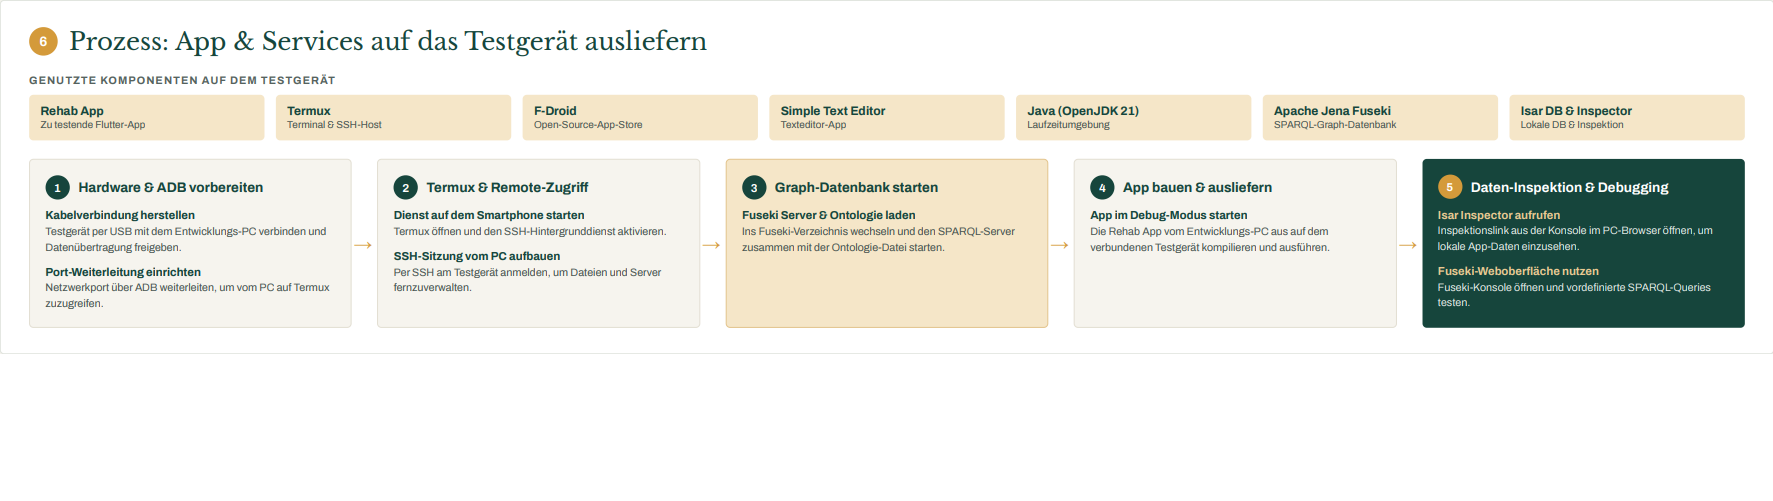
\includegraphics[width=0.8\textwidth]{bilder/API_3.png}
    \caption{Testaufbau mit physischem Smartphone}
    \label{fig:testaufbau}
\end{figure}

\section{Implementierung}

\subsection{Knowledge}

\subsubsection{Motivation und Zielsetzung}

Der Knowledge Graph dient der semantischen Modellierung
physiotherapeutischer Übungsdaten. Ziel ist es, Übungen
maschinenlesbar mit Körperteilen, Kategorien,
Schwierigkeitsgraden und Kontraindikationen zu verknüpfen,
um eine intelligente Empfehlungslogik zu ermöglichen.

\subsubsection{Ontologie-Design}

\paragraph{Verwendete Ontologie}

Als Basis wurde die \textit{Physical Therapy Ontologie}
(\texttt{http://purl.org/PhysicalTherapy}) verwendet und
durch projektspezifische Vokabulare erweitert.

\subsection{API und Datenhaltung}

\subsection{UI und Interaktion}

\subsection{Integration}

\section{Bewertung und Schluss}

\subsection{Erreichte Ziele}

Im Projekt wurde ein funktionsfähiger ReVia-Prototyp entwickelt, der die Ergebnisse der Nutzerstudie mit einer strukturierten Wissensbasis und einer mobilen Benutzeroberfläche verbindet. Zentrale Anforderungen wie verständliche Übungsdarstellungen, grundlegende Personalisierung, Fortschritts- und Schmerzverläufe sowie eine einfache Bedienung wurden in der Anwendung aufgegriffen.

Die Wissensbasis stellt dafür strukturierte Informationen zu Übungen, Körperregionen, Kontraindikationen, Trainingseffekten und weiteren rehabilitationsbezogenen Inhalten bereit. Über SPARQL-Abfragen und einen Fuseki-Server können diese Informationen von der Anwendung abgefragt werden. Nutzerspezifische Angaben und Verlaufsdaten werden lokal in einer Isar-Datenbank gespeichert und bei der Erstellung beziehungsweise Filterung von Trainingsplänen berücksichtigt.

Auch die technische Integration der Komponenten konnte umgesetzt und mit realen Daten getestet werden. Der entstandene Prototyp umfasst unter anderem ein Profil mit interaktiver Körperkarte, die Erstellung und Empfehlung von Trainingsplänen, Übungsansichten mit Anleitungen und ergänzenden Medien sowie Funktionen zur Dokumentation von Training, Schmerzen und Fortschritt. Damit wurde das zentrale Projektziel erreicht, Wissensmodellierung, technische Datenabfrage und nutzerzentrierte Gestaltung in einem gemeinsamen Prototyp zusammenzuführen.

\subsection{Herausforderungen und technische Entscheidungen}

Eine zentrale Herausforderung des Projekts war die enge Abhängigkeit zwischen Knowledge Graph, API und Benutzeroberfläche. Änderungen an der Ontologie konnten direkte Auswirkungen auf die Abfragen und damit auf die in der Anwendung verfügbaren Inhalte haben. Gleichzeitig entstanden aus der Gestaltung und Implementierung der Benutzeroberfläche neue Anforderungen an die Struktur der Wissensbasis.

Besonders deutlich wurden diese Abhängigkeiten bei Änderungen an der Modellierung der Körperregionen. Dabei zeigte sich, dass bereits kleinere Änderungen an gemeinsam verwendeten Begriffen oder Beziehungen dazu führen konnten, dass Inhalte in der Anwendung nicht mehr korrekt gefunden wurden. Die stärkere Nutzung der vorhandenen \texttt{partOf}-Beziehungen sowie Tests gegen einen lokal betriebenen Fuseki-Server machten die Integration robuster.

Eine weitere technische Entscheidung war die Trennung zwischen inhaltlichen Daten und nutzerspezifischen Daten. Rehabilitationsbezogene Inhalte wie Übungen und ihre Beziehungen werden im Knowledge Graph verwaltet, während persönliche Angaben, Trainingspläne und Verlaufsdaten lokal in Isar gespeichert werden. Dadurch konnte die Wissensbasis unabhängig von den individuellen Nutzerdaten gepflegt werden.

Der Projektverlauf zeigte insgesamt, dass für ein System mit mehreren eng verbundenen Komponenten klare Schnittstellen und regelmäßige gruppenübergreifende Tests notwendig sind. Die Qualität der Anwendung hängt nicht nur von der Implementierung einzelner Komponenten ab, sondern auch davon, dass Datenmodell, Abfragen und Benutzeroberfläche dieselben Strukturen und Begriffe verwenden.

\subsection{Limitationen}

Der aktuelle Stand von ReVia ist als Prototyp zu verstehen und besitzt mehrere fachliche und technische Grenzen. Nicht umgesetzt wurden insbesondere eine automatische Bewegungserkennung, eine zuverlässige Bewertung der Übungsausführung sowie eine medizinische Beurteilung von Schmerzen, Verletzungen oder Diagnosen. Solche Funktionen würden zusätzliche technische Verfahren und eine fachliche beziehungsweise medizinische Validierung erfordern.

Auch die Personalisierung ist im aktuellen Stand begrenzt. Die Auswahl von Übungen berücksichtigt bereits verschiedene Nutzerangaben und Eigenschaften aus der Wissensbasis, bildet jedoch keinen vollständigen individuellen Rehabilitationsverlauf ab. Heilungsphasen, Belastbarkeit oder Veränderungen des Zustands über längere Zeit werden noch nicht systematisch für die Freigabe oder Anpassung von Übungen verwendet.

Eine weitere Grenze liegt in der Vollständigkeit und Qualität der Wissensbasis. Nicht alle modellierten Inhalte verfügen bereits über sämtliche Angaben, die von den aktuellen API-Abfragen vorausgesetzt werden. Dadurch können einzelne Übungen, Alltagshinweise oder Rezepte trotz vorhandener Modellierung noch nicht vollständig von der Anwendung verarbeitet werden. Die Qualität personalisierter Empfehlungen hängt daher wesentlich von konsistenten, vollständigen und fachlich geprüften Daten ab.

ReVia ist zudem nicht als medizinisches Diagnose- oder Entscheidungssystem ausgelegt. Die Anwendung kann Fachpersonal nicht ersetzen und soll ausschließlich als unterstützendes Werkzeug für die selbstständige Rehabilitation zwischen Behandlungsterminen dienen.

\subsection{Erweiterungsmöglichkeiten}

Für eine Weiterentwicklung bietet insbesondere die Wissensbasis mehrere Ansatzpunkte. Medizinisch geprüfte Informationen zu Verletzungen und Krankheitsbildern könnten ergänzt und stärker mit Übungen, Kontraindikationen und Rehabilitationsphasen verknüpft werden. Auch die bereits vorbereitete Patient-Klasse könnte weiter ausgebaut werden, um zusätzliche Informationen strukturiert abzubilden.

Darüber hinaus könnte der individuelle Rehabilitationsverlauf stärker berücksichtigt werden. Übungen könnten beispielsweise abhängig von Heilungsphase, Trainingsstand und dokumentiertem Schmerzverlauf schrittweise freigegeben oder angepasst werden. Voraussetzung dafür wäre eine entsprechende Erweiterung der Wissensbasis und eine stärkere Verknüpfung dieser Informationen mit den lokal gespeicherten Nutzerdaten.

Auch bestehende Inhaltsbereiche können vervollständigt und erweitert werden. Beim Bereich ``Rezept der Woche'' fehlen bei einem Teil der bereits modellierten Einträge noch Angaben, die von der aktuellen API-Abfrage benötigt werden. Zusätzlich könnten Eigenschaften wie Zutaten, Kalorien oder Allergene ergänzt werden.

Weitere mögliche Erweiterungen sind differenziertere Fortschrittsdarstellungen, zusätzliche beziehungsweise eigene Übungsvideos sowie Kommunikations- und Zugriffsoptionen für Physiotherapeut:innen. Solche Funktionen müssten jedoch insbesondere im Hinblick auf Datenschutz, fachliche Verantwortung und den vorgesehenen Einsatzbereich der Anwendung genauer konzipiert werden.

\subsection{Diskussion / Reflexion}

Das Projekt zeigt, dass sich Nutzeranforderungen, semantische Wissensmodellierung und mobile Anwendungsentwicklung sinnvoll miteinander verbinden lassen. Die Nutzerstudie lieferte dabei eine wichtige Grundlage für die Auswahl und Gestaltung der Funktionen, während der Knowledge Graph die technischen Voraussetzungen für strukturierte und anpassbare Inhalte bereitstellte.

Gleichzeitig wurde deutlich, dass die organisatorische Aufteilung in einzelne Arbeitsbereiche nicht bedeutet, dass diese technisch unabhängig voneinander entwickelt werden können. Insbesondere zwischen Ontologie, API und Benutzeroberfläche entstanden wiederholt Abhängigkeiten. Änderungen an gemeinsam genutzten Begriffen oder Beziehungen mussten deshalb nicht nur innerhalb einer Gruppe, sondern im Gesamtsystem getestet werden. Der ursprünglich eher phasenweise geplante Ablauf entwickelte sich dadurch zu einem iterativen Prozess mit wiederholten Anpassungen.

Die Verwendung eines Knowledge Graphs ermöglichte es im Projekt, Beziehungen zwischen Übungen, Körperregionen, Einschränkungen und Trainingseffekten explizit abzubilden und über Abfragen nutzbar zu machen. Gleichzeitig macht dieser Ansatz die Datenqualität zu einem zentralen Bestandteil der Systemqualität. Fehlende oder inkonsistente Beziehungen wirken sich unmittelbar auf die Ergebnisse der Anwendung aus.

Im Austausch nach der Abschlusspräsentation wurde zudem deutlich, dass einzelne als Data Properties modellierte Inhalte alternativ als Individuals hätten abgebildet werden können. Dadurch wären bestimmte Informationen weniger statisch und teilweise besser wiederverwendbar gewesen. Diese Rückmeldung zeigt, dass auch die Wahl der Modellierungsform einen direkten Einfluss auf Erweiterbarkeit und Wiederverwendung innerhalb der Wissensbasis hat.

Der ReVia-Prototyp zeigt, wie sich der gewählte technische und konzeptionelle Ansatz innerhalb des Projektrahmens umsetzen lässt, stellt jedoch noch kein medizinisch validiertes Produkt dar. Für eine Weiterentwicklung wären neben technischer Verbesserung insbesondere eine systematische fachliche Prüfung der Inhalte, eine Bereinigung der verbleibenden Dateninkonsistenzen und eine weitergehende Evaluation mit Nutzer:innen und Fachpersonal erforderlich.

\subsection{Fazit}

Mit ReVia wurde im Rahmen des Bachelorprojekts ein Prototyp entwickelt, der Nutzeranforderungen, eine strukturierte Wissensbasis und die technische Umsetzung einer Reha-Anwendung miteinander verbindet. Ausgangspunkt war das Ziel, Patient:innen zwischen physiotherapeutischen Behandlungsterminen zu unterstützen, ohne medizinische Entscheidungen durch die Anwendung zu ersetzen.

Die Ergebnisse der Nutzerstudie wurden schrittweise in konkrete gestalterische und technische Lösungen überführt. Der Knowledge Graph stellt dafür strukturiertes Wissen bereit, die API übernimmt die Abfrage und Verarbeitung der Daten und die Benutzeroberfläche macht die daraus gewonnenen Informationen für die Nutzer:innen zugänglich. Der entstandene Prototyp deckt damit mehrere zentrale Nutzungsszenarien ab und zeigt, wie die Projektbereiche in einem gemeinsamen System zusammenwirken können.

Gleichzeitig bestehen klare Grenzen hinsichtlich Datenvollständigkeit, medizinischer Validierung und weitergehender Personalisierung. Gerade diese Punkte bieten jedoch konkrete Ansatzmöglichkeiten für eine zukünftige Weiterentwicklung.

Insgesamt bildet ReVia einen technischen und konzeptionellen Ausgangspunkt, auf dessen Grundlage sowohl die Integration der einzelnen Komponenten als auch die fachliche Qualität und Vollständigkeit der Wissensbasis in zukünftigen Entwicklungsphasen weiter verbessert werden können.



% Literaturverzeichnis
\clearpage
\printbibliography[heading=bibintoc]

\end{document}